%%%%%%%%%%%%%%%%%%%%%%%%%%%%%%%%%
% Bernoulli model
%%%%%%%%%%%%%%%%%%%%%%%%%%%%%%%%%

\section{Bernoulli set model}
\label{sec:bernoulli_model}
In the \emph{Bernoulli} set model, we describe the statistical properties of processes that \emph{generate} approximations of a certain kind that model many existing processes and generalizes to higher-order approximations under algebraic composition.

In what follows, we specify the axioms of the Bernoulli set model.

Theoretically, a process that generates approximations could exhibit correlations of any sort, but Bernoulli sets are constrained by the following axiom.
\begin{axiom}[Element-wise independence]
\label{asm:element_indep}
For all distinct $x, y \in U$, the error events at $x$ and $y$ are mutually independent:
\begin{equation}
P(\mathbf{1}_{\tilde{A}}(x) \neq \mathbf{1}_{A}(x) \mid \mathbf{1}_{\tilde{A}}(y) \neq \mathbf{1}_{A}(y)) =
	P(\mathbf{1}_{\tilde{A}}(x) \neq \mathbf{1}_{A}(x)).
\end{equation}
More generally, the family $\{\mathbf{1}_{\tilde{A}}(x) : x \in U\}$ is mutually independent given the objective set $A$ and the error rates.
Furthermore, within each partition block $B_i$ (\cref{def:model_order}), the error indicators $\{\mathbf{1}_{\tilde{A}}(x) : x \in B_i\}$ are identically distributed.
\end{axiom}

The complexity in the Bernoulli set model stems from the fact that different subsets of the universal set may exhibit different error rates.
Suppose the objective set $R \in 2^U$ induces a partition $\{B_1, \ldots, B_n\}$ of $U$ such that elements within each block $B_i$ share a common error rate $\alpha_i$.
\begin{definition}[Model order]
\label{def:model_order}
The \emph{order} of a Bernoulli set model is the number of partition blocks $n$.
A zeroth-order model ($n = 0$) is the degenerate case: no partition blocks and no errors (the exact set).
A first-order model ($n = 1$) assigns a single error rate to all elements (symmetric channel).
A second-order model ($n = 2$) distinguishes positives from negatives with rates $\tprate$ and $\fprate$ respectively.
In general, an $n$-th order model partitions $U$ into $n$ blocks, each with its own error rate; the maximum order is $|U|$.
\end{definition}
In the second-order (positive-negative) model, $n = 2$: the partition is $\{R, R^c\}$ with block response rates $\alpha_1 = \beta$ (response rate on positives, i.e., true positive rate) and $\alpha_2 = \alpha$ (response rate on negatives, i.e., false positive rate).
\begin{axiom}[Conditional independence of block error rates]
\label{asm:fpr_fnr_r_indep}
Given the objective set $R$, the random error rates $\alpha_1, \ldots, \alpha_n$ for the respective partition blocks $B_1, \ldots, B_n$ are mutually independent.
\end{axiom}
For instance, in the second-order model, the random false positive rate $\alpha$ and the random true positive rate $\beta$ are conditionally independent given $R$.

\begin{remark}[Relation to the binary symmetric channel]
\label{rem:bsc}
At the per-element level, the Bernoulli set model is a collection of independent binary symmetric channels~\cite{shannonBSC}; equivalently, each element undergoes Warner's randomized response~\cite{warner1965}. For each $x \in U$, the indicator $\mathbf{1}_{\tilde{A}}(x)$ is the output of a BSC with crossover probability $\fprate$ (if $x \notin A$) or $\fnrate$ (if $x \in A$).
The novelty of the present framework is not the per-element channel model, which is classical, but the \emph{set-level} compositional algebra: the derivation of error rates for union, intersection, complement, and their higher-order compositions over collections of such channels.
\end{remark}

\begin{remark}[Axiom economy]
\label{rem:axiom_economy}
Most results in this paper---the distributions of all binary classification measures (\cref{sec:characteristics}), the set-operation error rates and monoidal structure (\cref{sec:set_theory}), and the relational probabilities (\cref{sec:relational})---follow from \cref{asm:element_indep} alone.
\Cref{asm:fpr_fnr_r_indep} is needed only when the objective set $R$ is itself uncertain, in which case it permits the factorization of the joint distribution of $\tilde{R}$ and $R$ (\cref{sec:prob_model}) and the entropy decomposition (\cref{sec:entropy}).
\end{remark}

There are two natural \emph{statistics} of the Bernoulli set model, the random false positive and true positive rates conditioned on $R = A$.
They are respectively defined by
\begin{equation}
\label{def:sample_fprate}
	\alpha = \frac{1}{|A^c|} \sum_{x \in A^c} \mathbf{1}_{\tilde{A}}(x)
\end{equation}
and
\begin{equation}
\label{def:sample_tprate}
	\beta = \frac{1}{|A|} \sum_{x \in A} \mathbf{1}_{\tilde{A}}(x).
\end{equation}
\begin{proposition}
\label{prop:element_rates}
By \cref{asm:element_indep}, for any single element $x \notin A$,
$\Prob{\mathbf{1}_{\tilde{A}}(x) = 1} = \fprate$, and for $x \in A$,
$\Prob{\mathbf{1}_{\tilde{A}}(x) = 1} = \tprate$.
The expected sample rates satisfy $E[\alpha] = \fprate$ and $E[\beta] = \tprate$.
\end{proposition}



We denote the second-order random approximate set generative model by $\tilde{R}$, with random false positive rate $\alpha$ and random true positive rate $\beta$ conditioned on the objective set $R$.
The conditional distribution of $\tilde{R}$ given $R = X$ is denoted by $\tilde{X}$.
When the rates are degenerate, the model reduces to a deterministic outcome, e.g., $\tilde{A}$ given $\alpha = 0$ and $\beta = 1$ places all probability mass on $A$.

We parameterize $\tilde{X}$ by its expected false positive rate $\fprate$ and expected true positive rate $\tprate$, writing
\begin{equation}
\tilde{X}[\fprate][\tprate].
\end{equation}
We define the complementary rates $\fnrate = 1-\tprate$ (FNR) and $\tnrate = 1-\fprate$ (TNR) as shorthands that appear naturally in derived expressions.
Special cases with only one type of error specified are written $\tilde{X}[\fprate][-]$ and $\tilde{X}[+][\tprate]$.

Random \emph{positive} and \emph{negative} approximate sets are special cases respectively given by the following definitions.
\begin{definition}
\label{def:pos_approx_set}
A random approximate set $\tilde{A}[0][+]$ is a random \emph{positive} approximate set denoted by $\tilde{A}_+$.
\end{definition}
\begin{definition}
\label{def:neg_approx_set}
A random approximate set $\tilde{A}[-][0]$ is a random \emph{negative} approximate set denoted by $\tilde{A}_-$.
\end{definition}
By these definitions, every realization of $\tilde{A}_+$ and $\tilde{A}_-$ are respectively \emph{supersets} or \emph{subsets} of $A$.
The complement of a random positive (negative) approximate set is a random negative (positive) approximate set.

By \cref{asm:fpr_fnr_r_indep} and by the axioms of probability,
\begin{equation}
f(\tilde{X}, \alpha, \beta) =
f(\tilde{X} | \alpha, \beta)
f(\alpha | R) f(\beta | R).
\end{equation}

Every statistical property of the second-order random approximate set model is entailed by \cref{def:sample_fprate,def:sample_tprate}.
Furthermore, these assumptions generally hold in practice, e.g., the Bloom filter~\cite{bf} and Perfect hash filter~\cite{phf} are two separate implementations of the random positive approximate set in which these assumptions hold.

\subsection{Abstract data type}
\label{sec:adt}
A data type $T$ that overloads the membership predicate $\SetContains : U \times T \to \{0,1\}$ and has a value constructor $\ctor{\fprate}{\tprate} : 2^U \to T$ \emph{models} the Bernoulli set abstract data type if \cref{def:sample_fprate,def:sample_tprate} are satisfied, i.e.,
\begin{equation}
	\Prob{\SetContains[x][\ctor{\fprate}{\tprate}(A)] | \SetNotContains[x][A]} = \fprate
\end{equation}
and
\begin{equation}
	\Prob{\SetContains[x][\ctor{\fprate}{\tprate}(A)] | \SetContains[x][A]} = \tprate.
\end{equation}
Two data types that model Bernoulli sets with the same expected error rates are interchangeable in the frequentist sense: at the limit of repeated independent runs, they produce the same distribution over outcomes.

Suppose the second-order random approximate sets are over the universal set $U$.
Compositions of second-order random approximate sets over the Boolean algebra $(2^U,\cup,\SetIntersection,\SetComplement,\EmptySet,U)$, or random approximate sets of random approximate sets, are not closed over the \emph{second-order} model.
These compositions are addressed in the higher-order model below.

\subsection{Higher-order models and composition}
\label{sec:higher_order_model}

We compose \emph{random approximate sets} over the Boolean algebra $(\Sigma,\SetUnion,\SetIntersection,\SetComplement,\EmptySet,\Set{U})$, where $\Sigma \subseteq \PS{\Set{U}}$ because a deterministic implementation may not reach every element of $\PS{\Set{U}}$.
As a result, to satisfy the identity and complementation axioms required by Boolean algebras, we make $\EmptySet$ and $\Set{U}$ available in the model as special cases.
\begin{remark}
	Alternatively, these axioms may be satisfied by making the empty set and the universal set \emph{degenerate} cases, i.e., $\Prob{\ASet{\EmptySet} = \EmptySet} = 1$ and $\Prob{\ASet{U} = \Set{U}} = 1$.
\end{remark}

Furthermore, we may replace any of the operators in the Boolean algebra with \emph{random approximations} that model the noisy or rate-distorted channel previously described, i.e., these operators may themselves be constructors for random approximate sets, e.g., $\Set{A} \, \AT{\SetUnion}[\fprate][\tprate] \, \Set{B} \sim \AT{(\SetUnion[\Set{A}][\Set{B}])}[\tprate][\fprate]$ where $\AT{\SetUnion}[\fprate][\tprate]$ maps negatives to positives with probability $\fprate$ and maps positives to negatives with probability $\tprate$.

A natural mapping is provided by the \emph{identity} function $\Fun{id} \colon \PS{\Set{X}} \to \PS{\Set{X}}$, which is defined as
\begin{equation}
\Fun{id}(\Set{A}) \coloneqq \Set{A}\,.
\end{equation}
However, suppose we only have an \emph{approximation} of the identity function, denoted by $\APFun{id}[\fprate][\tprate]$, such that $\APFun{id}[\fprate][\tprate](\Set{A}) \sim \ASet{A}[\fprate][\tprate]$.
Then $\APFun{id}[\fprate][\tprate]$ generates sets consistent with the random approximate set model.

If we compose random approximate sets, then we have \emph{higher-order} random approximate sets.
\begin{theorem}
\label{thm:composition_rates}
	The composition of random approximate identity functions $\APFun{id}[\fprate][\tprate] \circ \APFun{id}[\fprate'][\tprate']$ generates random approximate sets with a true positive rate $\tprate' \tprate + \fnrate' \fprate$ and false positive rate $\fprate' \tprate + \tnrate' \fprate$.
\end{theorem}
\begin{proof}
	Let $x \in A$. In the inner approximation $\APFun{id}[\fprate'][\tprate']$, element $x$ tests positive with probability $\tprate'$ and negative with probability $\fnrate' = 1 - \tprate'$.
	In the outer approximation $\APFun{id}[\fprate][\tprate]$, a positive is retained with probability $\tprate$ and a negative is promoted to positive with probability $\fprate$.
	By the law of total probability, the composed true positive rate is
	$\tprate' \cdot \tprate + \fnrate' \cdot \fprate$.
	Similarly, let $x \notin A$. In the inner approximation, $x$ tests positive with probability $\fprate'$ and negative with probability $\tnrate' = 1 - \fprate'$.
	The composed false positive rate is
	$\fprate' \cdot \tprate + \tnrate' \cdot \fprate$.
\end{proof}

\begin{definition}
	The \emph{iterated} function $\Fun{f}^k$ is defined as $k$ compositions of $\Fun{f}$ where $\Fun{f}^0$ denotes the (non-random) \emph{identity} function.
\end{definition}
The composition $\left(\APFun{id}[\fprate][\tprate]\right)^k$ generates $k$-fold compositions of random approximate sets where the \emph{zero-th} order random approximation is the identity, i.e., $\left(\APFun{id}\right)^0 = \Fun{id}$.

The function being approximated may take other forms, like \emph{set-complementation} or \emph{set-union}, e.g.,
let $\SetUnion \colon \PS{\Set{X}} \times \PS{\Set{X}} \to \PS{\Set{X}}$ be approximated by $\APFun{\SetUnion}[\fprate][\tprate] \colon \PS{\Set{X}} \times \PS{\Set{X}} \to \PS{\Set{X}}$.
Then, $\Set{A} \APFun{\SetUnion}[\fprate][\tprate] \Set{B}$ is a random approximate set of $\SetUnion[\Set{A}][\Set{B}]$ as before.
However, $\APFun{\SetUnion}[\fprate'][\tprate'] \circ \APFun{id}[\fprate][\tprate]$ generates two-fold compositions of random approximate sets.

\begin{theorem}
\label{thm:twofold_composition}
	Given a random approximate set $\ASet{A}[\fprate_1][\tprate_1]$, a random approximation of $\ASet{A}[\fprate_1][\tprate_1]$ with a false positive rate $\fprate_2$ and true positive rate $\tprate_2$ is a \emph{two-fold composition} approximating $\Set{A}$ with a false positive rate $\fprate = \fprate_1 \tprate_2 + \tnrate_1 \fprate_2$ and true positive rate $\tprate = \tprate_1 \tprate_2 + \fnrate_1 \fprate_2$, denoted by $\Set{A}^{\sigma^2}(\tprate,\fprate)$.

	This result may be recursively applied to derive arbitrary $k$-fold compositions as given by
	\begin{equation}
		\Set{A}^{\sigma^k} = \left(\Set{A}^{\sigma^{k-1}}\right)^{\sigma}
	\end{equation}
	where the \emph{zero-th} order $\Set{A}^{\sigma^0} = \Set{A}$.
\end{theorem}
\begin{proof}
The result follows by applying \cref{thm:composition_rates} with inner
rates $(\fprate_1, \tprate_1)$ and outer rates $(\fprate_2, \tprate_2)$.
The recursive formula holds by induction: the base case $k = 0$ is the
exact identity, and the inductive step applies \cref{thm:composition_rates}
to the $k$-th order rates as inner parameters.
\end{proof}

\begin{figure}[ht]
\centering
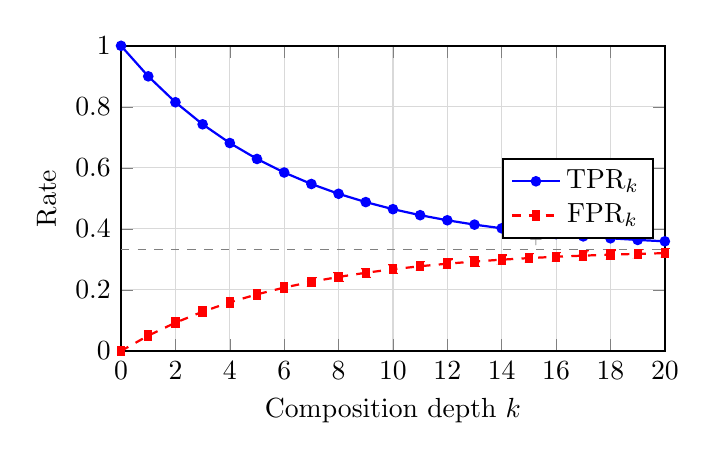
\begin{tikzpicture}
\begin{axis}[
	width=0.7\textwidth,
	height=0.45\textwidth,
	xlabel={Composition depth $k$},
	ylabel={Rate},
	xmin=0, xmax=20,
	ymin=0, ymax=1,
	legend style={at={(0.98,0.5)}, anchor=east},
	ymajorgrids, xmajorgrids,
	major grid style={gray!30},
	thick,
	xtick={0,2,...,20},
]
\addplot[blue, solid, mark=*, mark size=1.5pt] coordinates {
	(0,1.00000000) (1,0.90000000) (2,0.81500000)
	(3,0.74275000) (4,0.68133750) (5,0.62913688)
	(6,0.58476634) (7,0.54705139) (8,0.51499368)
	(9,0.48774463) (10,0.46458294) (11,0.44489550)
	(12,0.42816117) (13,0.41393700) (14,0.40184645)
	(15,0.39156948) (16,0.38283406) (17,0.37540895)
	(18,0.36909761) (19,0.36373297) (20,0.35917302)
};
\addlegendentry{TPR$_k$}
\addplot[red, dashed, mark=square*, mark size=1.5pt] coordinates {
	(0,0.00000000) (1,0.05000000) (2,0.09250000)
	(3,0.12862500) (4,0.15933125) (5,0.18543156)
	(6,0.20761683) (7,0.22647430) (8,0.24250316)
	(9,0.25612768) (10,0.26770853) (11,0.27755225)
	(12,0.28591941) (13,0.29303150) (14,0.29907678)
	(15,0.30421526) (16,0.30858297) (17,0.31229553)
	(18,0.31545120) (19,0.31813352) (20,0.32041349)
};
\addlegendentry{FPR$_k$}
\addplot[gray, thin, dashed, forget plot, domain=0:20] {1/3};
\node[anchor=west, gray] at (axis cs:14.5,0.37) {$\scriptstyle\frac{\fprate}{\fprate+\fnrate}$};
\end{axis}
\end{tikzpicture}
\caption{True positive rate and false positive rate under $k$-fold
composition of the approximate identity
$\APFun{id}[\fprate][\tprate]$ with $\fprate = 0.05$ and $\tprate = 0.90$.
Both rates converge to the stationary point
$\fprate/(\fprate + \fnrate) = 1/3$, where $\fnrate = 1 - \tprate$.
At high $k$, the approximation degrades toward a coin flip weighted by the
channel's stationary distribution.}
\label{fig:kfold_composition}
\end{figure}

In an \emph{algebra of sets} $(\PS{\Set{U}}, \SetIntersection, \SetUnion, \SetComplement, \Set{U}, \EmptySet)$, we may compose sets to form new sets.
When these sets model \emph{random approximate sets}, then their compositions model \emph{higher-order} random approximate sets, e.g.,
$\SetUnion[\ASet{A}[\fprate_1][\tprate_1]][\ASet{B}[\fprate_2][\tprate_2]]$
models a higher-order random approximate set which does not obey the second-order model; rather, it partitions the negative set such that each partition may have a different false positive rate and similarly for the positive set.

This contrasts with $\AT{\left(\SetUnion[\Set{A}][\Set{B}]\right)}[\fprate][\tprate]$, in which the false positive rate for the negative elements are uniformly distributed and likewise for the positive elements.
We call these random approximate sets \emph{second-order} approximations.
For completeness, the \emph{zeroth-order} are the objective sets, e.g., the zeroth-order approximation of $\SetUnion[\Set{A}][\Set{B}]$ is $\SetUnion[\Set{A}][\Set{B}]$.
The complexity of the probabilistic model increases as the order increases.

\subsection{Probability space}
\label{sec:prob_model}
The sample space is $\Omega = 2^U$, and the probability space is $(\Omega, \PS{\Omega}, P)$.
By \cref{asm:element_indep}, the conditional distribution of $\tilde{A}$ given the objective set $A$ factorizes element-wise:
\begin{equation}
    \Prob{\tilde{A} = S \Given A} = \prod_{x \in U} \Prob{\mathbf{1}_{\tilde{A}}(x) = \mathbf{1}_S(x) \Given \mathbf{1}_A(x)},
\end{equation}
where each factor equals $\tprate$ or $\fprate$ (if the element tests positive) or $\fnrate$ or $\tnrate$ (if it tests negative), depending on whether $x \in A$.

\begin{remark}[Latent and observed sets]
\label{rem:latent_observed}
The Bernoulli set model induces a duality between the \emph{latent} (objective) set $A$
and the \emph{observed} (approximate) set $\tilde{A}$.
Given the error model, the observed set constrains the possible latent sets.
For instance, if $\tilde{A}$ is a positive approximate set ($\fnrate = 0$),
then $A \subseteq \tilde{A}$: every element of $\tilde{A}$ is either a true positive
or a false positive, so the latent set must be a subset of the observed set.
Conversely, elements absent from $\tilde{A}$ are certainly absent from $A$.
\end{remark}


Consider the following example.
\begin{example}[Boolean universe]
\label{ex:boolean_universe}
	Let the universal set be $U = \{\top, \bot\}$ (the Boolean values \emph{true} and \emph{false}) and let the objective set be $A = \{\top\}$.
	A Bernoulli set $\tilde{A}^\fprate_\tprate$ over this universe has four possible outcomes, enumerated by the probability mass function
	\begin{equation}
	p_{\tilde{A}^\fprate_\tprate}(\Set{X}) =
	\begin{cases}
	\fnrate \cdot \tnrate & \Set{X} = \EmptySet,\\
	\fnrate \cdot \fprate & \Set{X} = \{\bot\},\\
	\tprate \cdot \tnrate & \Set{X} = \{\top\},\\
	\tprate \cdot \fprate & \Set{X} = \{\top, \bot\}.
	\end{cases}
	\end{equation}
	The outcome $\Set{X} = \{\top, \bot\}$ means both a true positive ($\top \in \tilde{A}$) and a false positive ($\bot \in \tilde{A}$) occurred.
	The outcome $\Set{X} = \{\bot\}$ means a false positive and a false negative occurred simultaneously.
	In the positive approximate set ($\fnrate = 0$), only $\Set{X} \in \{\{\top\}, \{\top, \bot\}\}$ are reachable, so $A \subseteq \tilde{A}$ with certainty.
\end{example}

\begin{remark}[Membership tests as Bernoulli Booleans]
\label{rem:membership_boolean}
For a Bernoulli set over an arbitrary universe $U$, the membership test $x \in \tilde{A}$ returns a Boolean value that is itself a Bernoulli approximation of the latent answer $x \in A$.
Consider a positive approximate set such as a Bloom filter, where $\fnrate = 0$.
If we query an element $x$ and observe $x \in \tilde{A}_+$, the result may be a false positive: $x$ might not belong to the latent set $A$.
If we observe $x \notin \tilde{A}_+$, the result is certainly a true negative: $x \notin A$.
Thus each membership query projects the set-level Bernoulli model onto the Boolean universe of \cref{ex:boolean_universe}, yielding a single Bernoulli Boolean whose error structure is inherited from the underlying set.
This pattern extends beyond data structures.
The Miller--Rabin primality test returns ``composite'' (certainly correct) or ``probably prime'' (false positive with probability at most $1/4$ per round), making its output a positive Bernoulli Boolean: the latent answer is $\{\text{prime}\}$ or $\{\text{composite}\}$, and the observed answer is a one-sided approximation with $\fnrate = 0$ and $\fprate \leq 1/4$.
More generally, any randomized decision procedure with one-sided error produces Bernoulli Booleans.
\end{remark}

%%%%%%%%%%%%%%%%%%%%%%%%%%%%%%%%%
